\documentclass[11pt, a4paper]{scrartcl}

\usepackage[utf8]{inputenc}
\usepackage[T1]{fontenc}
\usepackage[english]{babel}
\usepackage{csquotes}

\usepackage{hyperref}
\hypersetup{
	colorlinks=true,
	linkcolor=black!19!blue,
	citecolor=black!19!blue,
	urlcolor=black!19!blue
}

\usepackage{graphicx}
\graphicspath{ {img/} }

\usepackage{enumerate}


\newcommand{\todo}[1]{\begin{enumerate}[align=left]
        \item [\textcolor{red}{\textbf{TODO:} }] \textcolor{red}{#1}
    \end{enumerate}
    } % TODO remove


\begin{document}

\begin{title}

    \begin{center}
        
\includegraphics[width=0.4\textwidth]{tu_logo.pdf}

        \vspace*{2em}
        \LARGE
        Extended Berkeley Packet Filter in the context of Industrial Internet of
        Things at the Edge

        \vspace*{1em}
        \small
        Bachelor's Thesis Proposal

        \vspace*{1em}
        Aurel Weinhold, 403779, a.weinhold@campus.tu-berlin.de

        \vspace*{1em}
        \today

    \end{center}

\end{title}


% content
\section{Motivation}

% IIoT
As industrial factories become larger and more connected, the demand for a
decentralized distributed system consisting of sensors, controllers and
compute-nodes grows larger.

The Industrial Internet of Things, as defined by
\citeauthor{boyes_industrial_2018}, is the aggregation of networked sensors and
actuators with optional cloud or edge computing platforms which enable real
time, intelligent, and autonomous access, collection, analysis, and
communications, of process, product and service information, within the
industrial environment~\cite{boyes_industrial_2018}. In this context
\enquote{industrial} refers to manufacturing and excludes mining, construction
and energy~\cite{noauthor_industry_nodate}.

% real-time
Some of these sensors and actuators also exhibit real-time behavior, to ensure
safety and Quality of Service (QoS). Real-time operation is defined by DIN 44300
to be the operation of a computer system with programs that are at any time
ready to process data in a way that the computational results are available
within a given period of time. This is necessary as these actors interact with
the real world, being in physical contact with each other and possible even
humans. To mitigate risk for human workers and to ensure QoS in the product it
is strictly necessary to be dependable, as a violation might cost millions or
potentially the lives of humans.
%\todo{Add actual source.}
%\todo{predictability}

% edge
As latencies in unknown networks are unpredictable a shift away from the cloud
towards the IIoT networks has been made. This edge computing, a new paradigm in
distributed systems, has introduced the idea to (pre-)compute \enquote{on the
edge} of the cloud~\cite{shi_edge_2016}, which significantly reduces response
times by avoiding these network latencies, all the while also reducing stress on
networks to and from the cloud and the computing resources of the cloud.

%\todo{Is global market actually IIoT? Is this relevant?}
%According to \citeauthor{placek_industrial_nodate} the global market for IIoT is
%expected to grow almost five-fold up to 2028~\cite{placek_industrial_nodate} and
%with it there will be an increase in demand for networking and controlling
%resources. To combat this fast increase, edge computing, a new paradigm in
%distributed systems, has introduced the idea to (pre-)compute \enquote{on the
%edge} of the cloud~\cite{shi_edge_2016}, which significantly reduces stress on
%the network and on the compute-resources of the cloud itself, while also
%allowing for faster response times by avoiding congested
%networks~\cite{shi_edge_2016}.

\section{Problem Statement}


\section{Approach}

%\todo{sources}
As Linux is widely supported by most consumer hardware, this approach also gives
the flexibility of choosing fitting hardware, without the need to inquire
expensive custom hardware and firmware.

% eBPF
Extended Berkeley Packet Filter (eBPF) is a flexible virtual machine in the
Linux kernel programmable during runtime from user space. It allows for simple
rather restricted programs to be safely executed in the kernel space at various
hook points.

%These simple programs may be written in a subset of C and then compiled into
%eBPF instructions, but similar to assembly, it is entirely possible to write the
%programs in eBPF instructions yourself. When loaded into the kernel, they are
%tested by the in-kernel verifier. This verifier checks the program against a set
%of restrictions including a limitation on the number of (eBPF) instructions and
%that there are not loops in the
%program\footnote{\url{https://www.kernel.org/doc/html/latest/bpf/verifier.html},
%accessed \formatdate{7}{6}{2022}} to ensure the safety of the kernel. Some of
%these restrictions however can be circumvented without diminishing the safety of
%the kernel.
%\todo{Rewrite part about loops.}

% How is eBPF used? What can be achieved?
Traditional usage of classic Berkeley Packet Filter (cBPF) was limited to
network applications, hooking into the eXpress Data Path (XDP), or the traffic
control (TC) stage of the Linux Kernel Network Stack to allow inspection and
filtering of packets early on in the pipeline. Although limited it opened to
door into advanced network level monitoring on the kernel level.

Only with its extension to eBPF in recent years, researchers have tried to use
it for more advanced network related tasks~\cite{miano_creating_2018} and even
completely different applications hooking into systemcalls.

%This thesis explores the possibilities in enhancing near real-time behavior by
%using and abusing(?) eBPF on the edge of an IIoT network to
%%select tasks based on a priority model and the load of the edge device.
%respond to certain requests with pre-computed responses (?) and by that increase
%response-time and decrease unnecessary computational stress on the edge node.

In this thesis we will introduce a framework using eBPF to enhance near
real-time behavior by decreasing the response time of the aforementioned simple
requests by avoiding the user space, and therefor context switches and
inefficient scheduling, as shown in Figure~\ref{fig:communication_after}. To
achieve this, a filter is going to be designed which detects the type of packet
received and decides based on criteria whether that request is to be handled by
the original user space program, i.e. it needs more advanced processing or
access to resources outside of the edge server, or to be directly replied to
inside the kernel from a further eBPF program.

This framework will be validated by recreating the scenario with real hardware.
There will be two set ups, one where repetitive tasks are handled in the user
space, where it would originally have been handled, and one where they are
handled in the kernel using eBPF. This allows to measure actual data, like the
response time and load of the edge server. Based on that data it is possible to
compare the two methods and evaluate the approach.


\begin{figure}[htpb]
       \centering
       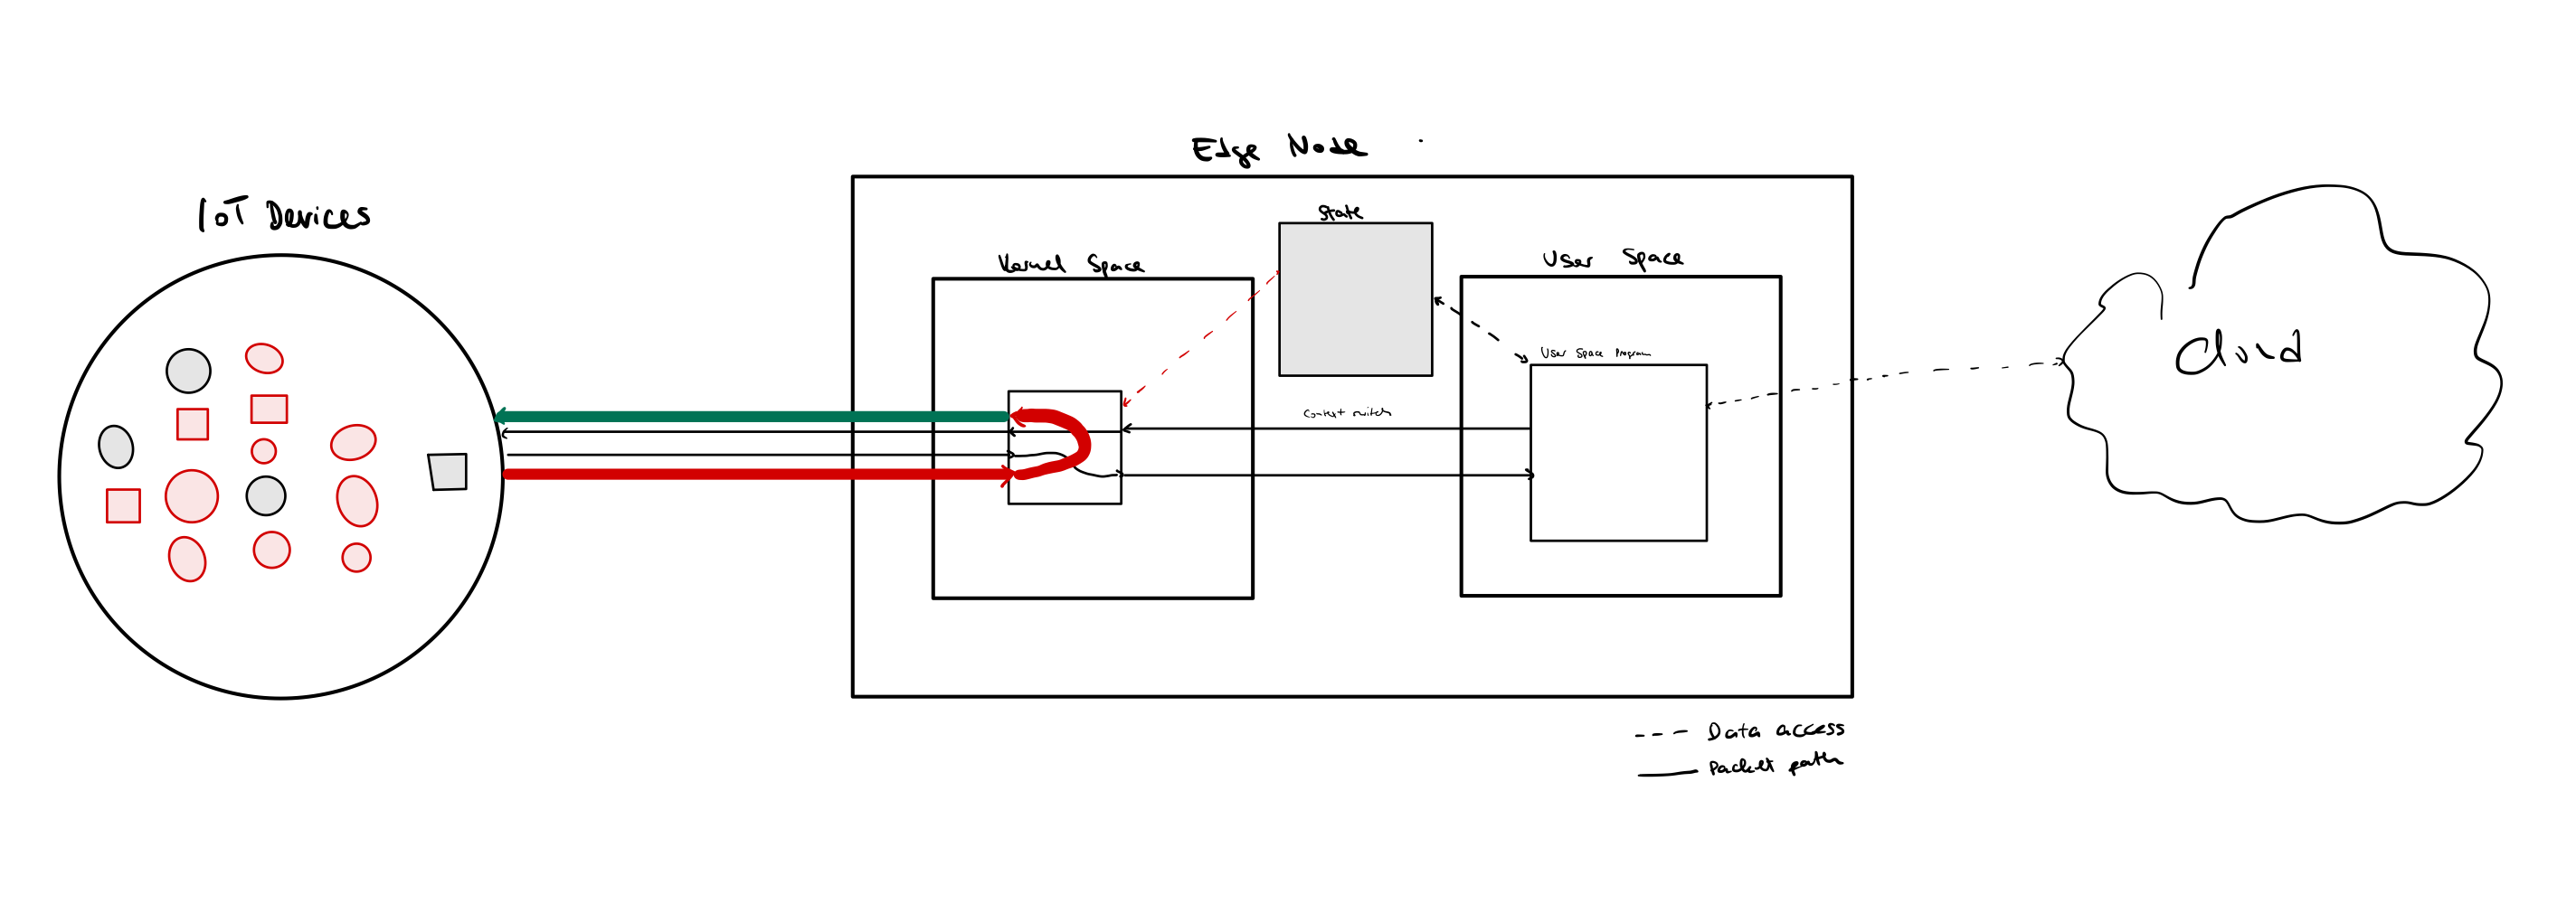
\includegraphics[width=\linewidth]{communication_after}
       \caption{communication after%
       \label{fig:communication_after}}%
\end{figure}

% \content


\end{document}
